%% Le lingue utilizzate, che verranno passate come opzioni al pacchetto babel. Come sempre, l'ultima indicata sar� quella primaria.
%% Se si utilizzano una o pi� lingue diverse da "italian" o "english", leggere le istruzioni in fondo.
\def\thudbabelopt{english}
%% Valori ammessi per target: bach (tesi triennale), mst (tesi magistrale), phd (tesi di dottorato).
%% --- Beamer ---
%% La chiave "beamer" attiva la modalit� slide e specifica le opzioni da passare all'omonima classe.
%% Le opzioni specificate "noamsthm,10pt" sono solamente indicative.
%% L'uso dell'opzione "ignorenonframetext" pu� creare problemi ed � quindi sconsigliato.
%% Se incontrate problemi con altre opzioni di "beamer" fatecelo sapere.
\documentclass[beamer={10pt,xcolor=dvipsnames},target=mst]{thud}

\usepackage{amsmath}
\usepackage{amssymb}
\usepackage{amsthm}
\usepackage{xcolor}
\usepackage{tikz}
\usepackage{adjustbox}
\usepackage{booktabs}
\usepackage{tabularx}
\usepackage[center]{caption}
\usepackage{mathtools}
\usepackage{stmaryrd}
\usepackage{subfig}
\usepackage{bm}


\usetikzlibrary{automata,positioning,shapes.multipart}

\makeatletter
\pgfdeclareshape{xor}
{
  \inheritsavedanchors[from=circle] 
  \inheritanchorborder[from=circle]
  \inheritanchor[from=circle]{north}
  \inheritanchor[from=circle]{north west}
  \inheritanchor[from=circle]{north east}
  \inheritanchor[from=circle]{center}
  \inheritanchor[from=circle]{west}
  \inheritanchor[from=circle]{east}
  \inheritanchor[from=circle]{mid}
  \inheritanchor[from=circle]{mid west}
  \inheritanchor[from=circle]{mid east}
  \inheritanchor[from=circle]{base}
  \inheritanchor[from=circle]{base west}
  \inheritanchor[from=circle]{base east}
  \inheritanchor[from=circle]{south}
  \inheritanchor[from=circle]{south west}
  \inheritanchor[from=circle]{south east}
  \inheritbackgroundpath[from=circle]
  \foregroundpath{
    \centerpoint%
    \pgf@xc=\pgf@x%
    \pgf@yc=\pgf@y%
    \pgfutil@tempdima=\radius%
    \pgfmathsetlength{\pgf@xb}{\pgfkeysvalueof{/pgf/outer xsep}}%  
    \pgfmathsetlength{\pgf@yb}{\pgfkeysvalueof{/pgf/outer ysep}}%  
    \ifdim\pgf@xb<\pgf@yb%
      \advance\pgfutil@tempdima by-\pgf@yb%
    \else%
      \advance\pgfutil@tempdima by-\pgf@xb%
    \fi%
    \pgfpathmoveto{\pgfpointadd{\pgfqpoint{\pgf@xc}{\pgf@yc}}{\pgfqpoint{\pgfutil@tempdima}{0pt}}}
    \pgfpathlineto{\pgfpointadd{\pgfqpoint{\pgf@xc}{\pgf@yc}}{\pgfqpoint{-\pgfutil@tempdima}{0pt}}}
    \pgfpathmoveto{\pgfpointadd{\pgfqpoint{\pgf@xc}{\pgf@yc}}{\pgfqpoint{0pt}{-\pgfutil@tempdima}}}
    \pgfpathlineto{\pgfpointadd{\pgfqpoint{\pgf@xc}{\pgf@yc}}{\pgfqpoint{0pt}{\pgfutil@tempdima}}}
    \pgfsetarrowsstart{}
    \pgfsetarrowsend{}
  }
}
\makeatother


%\usetheme{metropolis} 
\definecolor{UBCblue}{rgb}{0.04706, 0.13725, 0.46667} % UBC Blue (primary)

\usecolortheme[named=UBCblue]{structure}
\setbeamertemplate{navigation symbols}{}
\setbeamertemplate{footline}[frame number]

\setbeamerfont{bibliography item}{size=\scriptsize}
\setbeamerfont{bibliography entry author}{size=\scriptsize}
\setbeamerfont{bibliography entry title}{size=\scriptsize}
\setbeamerfont{bibliography entry location}{size=\scriptsize}
\setbeamerfont{bibliography entry note}{size=\scriptsize}

%% --- Informazioni sulla tesi ---
%% Per tutti i tipi di tesi
\title{Cryptographic Primitives for Zero-Knowledge: Theory and Implementation}
\author{Stefano Trevisani}
\course{Artificial Intelligence and Cybersecurity}
\supervisor{Dr.\ Arnab Roy}
\cosupervisor{Prof.\ Alberto Policriti\and Prof.\ Elisabeth Oswald}
\tutor{M.Sc.\ Matthias Steiner}

%% Altri campi disponibili: \tutor, \date (anno accademico, calcolato in automatico).
%% Con \supervisor, \cosupervisor e \tutor si possono indicare pi� nomi separati da \and.
%% Per le sole tesi di dottorato
%\cycle{XXVIII}
%% Campi obbligatori: \title, \author e \course.

%% Nel resto del preambolo potete personalizzare la presentazione liberamente.
%% Se incontrate problemi causati dall'interazione tra "thud" e "beamer" fatecelo sapere.

\newcommand{\Stamp}{\texttt{Stamp}}
\newcommand{\Blocc}{\texttt{Blocc}}
\newcommand{\abs}[1]{\left\lvert#1\right\rvert}
\newcommand{\gengroup}[1]{\left\langle#1\right\rangle}
\newcommand{\bitand}{\mathbin{\textnormal{\textsc{and}}}}
\newcommand{\bitxor}{\mathbin{\textnormal{\textsc{xor}}}}
\newcommand{\algid}{\mathrm{e}}
\newcommand{\Endset}[1]{\mathrm{End}\left(#1\right)}
\newcommand{\Set}[1]{\left\{#1\right\}} %chktex 21
\newcommand{\Tuple}[1]{\left(#1\right)} %chktex 21
\newcommand{\fooid}{\mathrm{id}}


\begin{document}

%% Il frontespizio prima di tutto!
%% \maketitle accetta gli stessi argomenti opzionali di \begin{frame} (p.es. "[plain]")
\maketitle

\begin{frame}{Verifiable Computation}
  \begin{figure}
    \centering
    \href{https://www.template.net/editable/illustrations}{
      \includegraphics[scale=0.0625]{res/cloud_computing.pdf}}
  \end{figure}

  \emph{Verifiable computation}:
  \begin{itemize}
    \item \textcolor{teal}{Server}: computes some function.
    \item \textcolor{orange}{Client(s)}: verify the correctness of the results.
  \end{itemize}
  \vspace*{16pt}
  Many applications:
  \begin{itemize}
    \item Delegating heavy loads to the cloud~\cite{AndersonCKLW2002}.
    \item Calculating household due bills~\cite{ParnoGHR2013}.
    \item \textbf{Verifying transactions on the blockchain.}~\cite{SassonCGGMTV2014}
  \end{itemize}
\end{frame}

%% Diapositiva
\begin{frame}{Interactive Proof Systems~\cite{GoldwasserMR1989}}
  \begin{figure}
    \centering
    \adjustbox{max height=96pt,keepaspectratio}
    {
    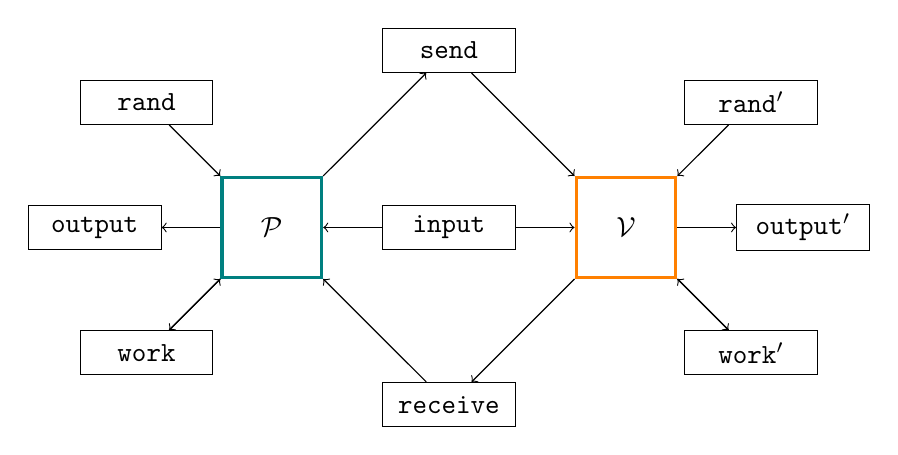
\begin{tikzpicture}[node distance=64pt,on grid,auto]
      \node[state,shape=rectangle,minimum height=16pt, minimum width=48pt] (in)  {\(\mathtt{input} \)};
      \node[state,shape=rectangle,very thick,draw=teal,minimum size=36pt,left =of in]   (m0)         {\(\mathcal{P}\)};
      \node[state,shape=rectangle,very thick,draw=orange,minimum size=36pt,right =of in] (m1)  {\(\mathcal{V}\)};
      \node[state,shape=rectangle,minimum height=16pt, minimum width=48pt,above left =of m0] (p0)  {\(\mathtt{rand}\)};
      \node[state,shape=rectangle,minimum height=16pt, minimum width=48pt,above right =of m1] (p1)  {\(\mathtt{rand}' \)};
      \node[state,shape=rectangle,minimum height=16pt, minimum width=48pt,below left =of m0] (w0)  {\(\mathtt{work} \)};
      \node[state,shape=rectangle,minimum height=16pt, minimum width=48pt,below right =of m1] (w1)  {\(\mathtt{work}' \)};
      \node[state,shape=rectangle,minimum height=16pt, minimum width=48pt,above =of in] (s0)  {\(\mathtt{send} \)};
      \node[state,shape=rectangle,minimum height=16pt, minimum width=48pt,below =of in] (r0)  {\(\mathtt{receive} \)};
      \node[state,shape=rectangle,minimum height=16pt, minimum width=48pt,left =of m0] (o0)  {\(\mathtt{output} \)};
      \node[state,shape=rectangle,minimum height=16pt, minimum width=48pt,right =of m1] (o1)  {\(\mathtt{output}' \)};
      \path[->]
      (in) edge (m0)
      (in) edge (m1)
      (p0) edge (m0)
      (p1) edge (m1)
      (w0) edge (m0)
      (m0) edge (w0)
      (w1) edge (m1)
      (m1) edge (w1)
      (m0) edge (s0)
      (s0) edge (m1)
      (m1) edge (r0)
      (r0) edge (m0)
      (m0) edge (o0)
      (m1) edge (o1)
      ;
    \end{tikzpicture}
    }
  \end{figure}
  \vspace*{16pt}
  A pair of \textbf{interactive probabilistic Turing machines}:
  \begin{itemize}
    \item \textcolor{teal}{Prover}: wants to prove a statement by creating a proof.
    \item \textcolor{orange}{Verifier}: wants to check the soundness of the proof.
    \item \textcolor{orange}{Verifier} is PTIME, might be fooled with negligible probability.
    \item \textsc{IP} = \textsc{PSPACE}~\cite{Shamir1992}.
  \end{itemize}
\end{frame}

\begin{frame}{ZK-SNARK systems}
  \begin{figure}
    \centering
      \includegraphics[scale=0.25]{res/Zero-Knowledge-Proofs-Properties.pdf}
  \end{figure}

  ZK-SNARK systems:
  \begin{itemize}
    \item \textcolor{orange}{Verifier} might be curious \(\implies \) \textbf{Zero-Knowledge}.
    \item Verification must be fast \(\implies \) \textbf{Succinct}.
    \item There may be many verifiers  \(\implies \) \textbf{Non-interactive}.
    \item \textcolor{teal}{Prover} is polynomially bounded \(\implies \) \textbf{Argument of Knowledge}.
  \end{itemize}
  \vspace*{16pt}
  \textbf{Complexity dominated by proof generation time}.
\end{frame}

\begin{frame}{SNARKs via QAPs~\cite{GennaroGPR2012,ParnoGHR2013,Groth2016}}
  \begin{figure}
    \centering
      \includegraphics{res/pinocchio.pdf}
  \end{figure}
  \vspace*{16pt}
%  Setting up a SNARK for some computable function:
  Bounded computations via \emph{arithmetic circuits} over \(\mathbb{F}_p\):
  \begin{enumerate}
    \item \emph{Rank-1 constraint systems (\textbf{R1CS})} encode circuit invariants.
    \item \emph{Quadratic Arithmetic Programs (\textbf{QAP})} ``compress'' R1CSs.
    \item \textcolor{teal}{Prover}/\textcolor{orange}{Verifier} keys to build/check the proof: ensure integrity.
    \item Exploit bilinear maps, work in the exponent: discrete \(\log \) is hard!
    \item ``Inject'' randomness in the polynomials to get zero-knowledge.
  \end{enumerate}
  \vspace*{16pt}
  \textbf{Complexity depends on the number of R1CS constraints}.
%  \vspace*{16pt}
%  Generating the keys incurs into the \emph{toxic waste} problem\dots
\end{frame}

\begin{frame}{The Blockchain}
  \begin{figure}
    \centering
    \adjustbox{max height=128pt,keepaspectratio}{
    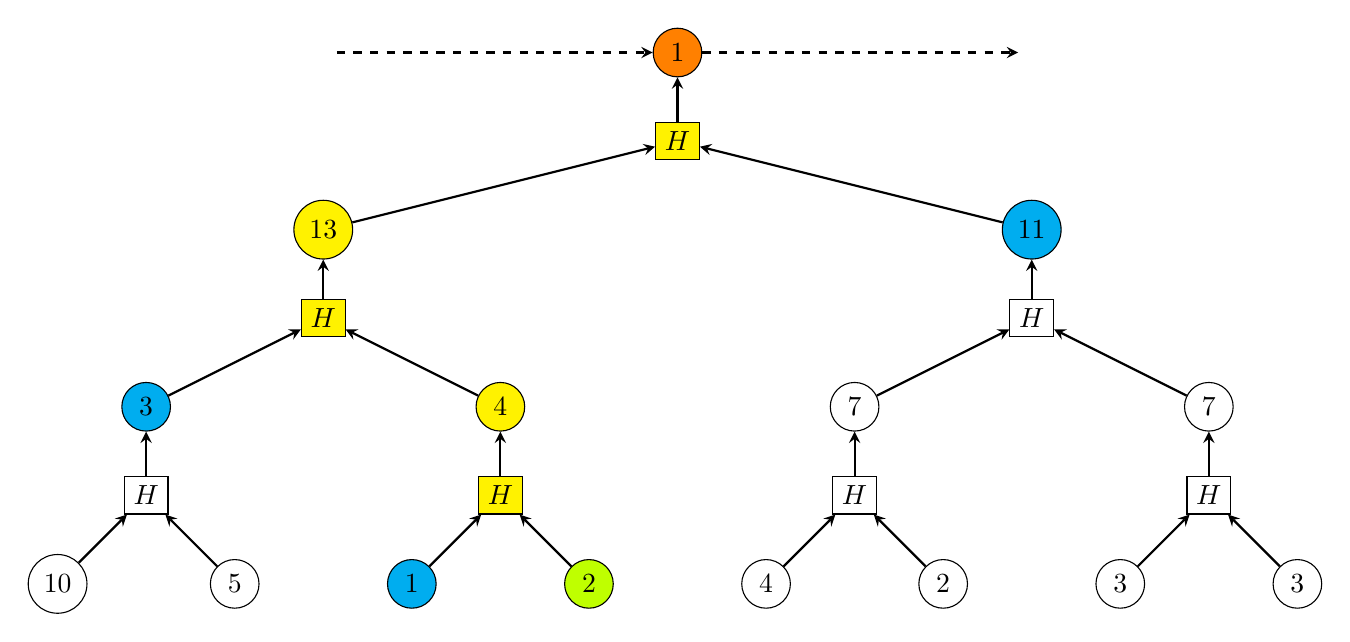
\begin{tikzpicture}[node distance={32pt}, node/.style = {draw, circle},on grid=true]
      \node[node] (y1) {\(10\)};
      \node[node,draw=none] (m1) [right of=y1] {};
      \node[node] (y2) [right of=m1] {\(5\)};
      \node[node,draw=none] (m2) [right of=y2] {};
      \node[node,fill=cyan] (y3) [right of=m2] {\(1\)};
      \node[node,draw=none] (m3) [right of=y3] {};
      \node[node,fill=lime] (y4) [right of=m3] {\(2\)};
      \node[node,draw=none] (m4) [right of=y4] {};
      \node[node] (y5) [right of=m4] {\(4\)};
      \node[node,draw=none] (m5) [right of=y5] {};
      \node[node] (y6) [right of=m5] {\(2\)};
      \node[node,draw=none] (m6) [right of=y6] {};
      \node[node] (y7) [right of=m6] {\(3\)};
      \node[node,draw=none] (m7) [right of=y7] {};
      \node[node] (y8) [right of=m7] {\(3\)};

      \node[node,shape=rectangle] (d1) [above of=m1] {\(H\)};
      \node[node,draw=none] (m8) [above of=m2] {};
      \node[node,shape=rectangle,fill=yellow] (d2) [above of=m3] {\(H\)};
      \node[node,draw=none] (m9) [above of=m4] {};
      \node[node,shape=rectangle] (d3) [above of=m5] {\(H\)};
      \node[node,draw=none] (m10) [above of=m6] {};
      \node[node,shape=rectangle] (d4) [above of=m7] {\(H\)};

      \node[node,fill=cyan] (x1) [above of=d1] {\(3\)};
      \node[node,draw=none] (n1) [above of=m8] {};
      \node[node,fill=yellow] (x2) [above of=d2] {\(4\)};
      \node[node,draw=none] (n2) [above of=m9] {};
      \node[node] (x3) [above of=d3] {\(7\)};
      \node[node,draw=none] (n3) [above of=m10] {};
      \node[node] (x4) [above of=d4] {\(7\)};
      \node[node,shape=rectangle,fill=yellow] (c1) [above of=n1] {\(H\)};
      \node[node,shape=rectangle] (c2) [above of=n3] {\(H\)};

      \node[node,fill=yellow] (x5) [above of=c1] {\(13\)};
      \node[node,draw=none] (n3) [above of=n2] {};
      \node[node,draw=none] (n4) [above of=n3] {};
      \node[node,fill=cyan] (x6) [above of=c2] {\(11\)};
      \node[node,shape=rectangle,fill=yellow] (c3) [above of=n4] {\(H\)};

      \node[node,fill=orange] (x7) [above of=c3] {\(1\)};
      \node[node,draw=none] (n5) [left =128pt of x7] {};
      \node[node,draw=none] (n6) [right =128pt of x7] {};


      \draw[-stealth,thick] (y1) to (d1);
      \draw[-stealth,thick] (y2) to (d1);
      \draw[-stealth,thick] (y3) to (d2);
      \draw[-stealth,thick] (y4) to (d2);
      \draw[-stealth,thick] (y5) to (d3);
      \draw[-stealth,thick] (y6) to (d3);
      \draw[-stealth,thick] (y7) to (d4);
      \draw[-stealth,thick] (y8) to (d4);

      \draw[-stealth,thick] (d1) to (x1);
      \draw[-stealth,thick] (d2) to (x2);
      \draw[-stealth,thick] (d3) to (x3);
      \draw[-stealth,thick] (d4) to (x4);


      \draw[-stealth,thick] (x1) to (c1);
      \draw[-stealth,thick] (x2) to (c1);
      \draw[-stealth,thick] (x3) to (c2);
      \draw[-stealth,thick] (x4) to (c2);

      \draw[-stealth,thick] (c1) to (x5);
      \draw[-stealth,thick] (c2) to (x6);

      \draw[-stealth,thick] (x5) to (c3);
      \draw[-stealth,thick] (x6) to (c3);

      \draw[-stealth,thick] (c3) to (x7);

      \draw[dashed,-stealth,thick] (n5) to (x7);
      \draw[dashed,-stealth,thick] (x7) to (n6);
    \end{tikzpicture}
    }
  \end{figure}

  \begin{itemize}
    \item Groups of transactions are leaves of a \textbf{Merkle tree}~\cite{Merkle1988}.
    \item Bottom-up computation using an \textbf{hash function}.
    \item The root contains a binding commitment.
    \item Check commitment via the short authentication path.
  \end{itemize}
\end{frame}

\begin{frame}{SHA~\cite{Dang2015}}
  \begin{figure}
    \centering
    \includegraphics[scale=0.175]{res/SHA-2.pdf}
  \end{figure}

  Standard designs, like SHA, are designed over \emph{boolean fields}:
  \begin{itemize}
    \item Bitwise AND, XOR, rotation, modulo \(2^{k}\) addition\dots
    \item Extremely efficient hardware and software implementations.
    \item However, ZK-SNARKs work over prime fields \(\implies \) emulation.
    \item SHA-256 \(\approx \) \textbf{25000 R1CS constraints}.
  \end{itemize}
\end{frame}

\begin{frame}{Arithmetization Oriented Primitives}
  \begin{figure}
    \centering
    \includegraphics[scale=1.0]{res/HoevenL2019.pdf}
  \end{figure}

  \emph{Arithmetization-Oriented} (AO) cryptographic primitives over \(\mathbb{F}_p\):
  \begin{itemize}
    \item Use only field \textbf{sum} and \textbf{multiplication}.
    \item Can be modeled as polynomials.
    \item Security depends on the feasibility of \textbf{algebraic attacks}.
  \end{itemize}
\end{frame}

\begin{frame}{\Mimc{}~\cite{AlbrechtGRRT2016}}
  \begin{figure}
    \centering
    \includegraphics[scale=0.75]{res/AlbrechtGRRT2016.pdf}
  \end{figure}

  \begin{itemize}
    \item \Mimc{}: Minimal Multiplicative Complexity.
    \item Extremely simple: \emph{round function} is \(x^3 + c\).
    \item Exponent is the lowest integer in \(\mathbb{F}_p\) coprime with \(p - 1\).
    \item \(\Ceil{\frac{\call{\log}{p}}{\call{\log}{3}}}\) rounds to achieve \textbf{degree overflow}.
    \item \Mimc-256: \textbf{640 R1CS constraints} (\(40\times \) less than SHA-256).
  \end{itemize}  
\end{frame}

\begin{frame}{\Poseidon{}~\cite{GrassiKRRS2021}}
  \begin{figure}
    \centering
    \includegraphics[scale=0.6]{res/GrassiKRRS2021.pdf}
  \end{figure}

  \begin{itemize}
    \item \Poseidon{}: \emph{substitution-permutation network} (from AES~\cite{DaemenR1999}).
    \item Full rounds defend against classic attacks.
    \item \textbf{Partial rounds} defend against algebraic attacks.
    \item \Poseidon{}-256: \textbf{240 R1CS constraints} (\(2.5\times \) less than \Mimc).
  \end{itemize}
\end{frame}

\begin{frame}{\Griffin{}~\cite{GrassiHRSWW2022}}
  \begin{figure}
    \centering
    \includegraphics[scale=0.75]{res/GrassiHRSWW2022.pdf}
  \end{figure}

  \begin{itemize}
    \item \Griffin{}: based on the \Horst{} scheme: \(\Tuple{x, y} \mapsto \Tuple{y, x \otimes \call{G}{y}}\).
    \item Circulant MDS matrix in the linear layer.
    \item Inverse power to achieve faster degree growth~\cite{AlyABDS2019}.
    \item \Griffin{}-256: \textbf{96 R1CS constraints} (\(2.5\times \) less than \Poseidon{}).
  \end{itemize}
\end{frame}

\begin{frame}{The GTDS~\cite{RoyS2022}}
  The new \emph{Generalized Triangular Dynamical System} (GTDS):
  \begin{center}
    \begin{align*}
      & x_{i} \;\;\;\; \longmapsto \;\;\;\; y_i = x_i^{d_1}\call{g_i}{\sum_{j=i+1}^{n}{x_j + y_j}} + \call{h_i}{\sum_{j=i+1}^{n}{x_j + y_j}}  \\
      & x_{n} \;\;\;\; \longmapsto \;\;\;\; y_n = x_{n}^{1/d_2} \\
      & \call{g_i}{x} = x^2 + \alpha_{i}x + \beta_{i} \\ 
      & \call{h_i}{x} = x^2 + \gamma_{i}x
    \end{align*}
  \end{center}

  \begin{itemize}
    \item Algebraic framework to design secure permutations.
    \item Encompasses existing strategies (Feistel, \Horst{}, SPN\dots).
    \item Extends previous designs, allows more flexibility. 
    \item \textbf{High degree permutation} representable using a \textbf{small R1CS}!
  \end{itemize}
\end{frame}

\begin{frame}{\Arion{} and \Arionp{}~\textbf{\cite{RoyST2023}}}
  \begin{figure}
    \centering
    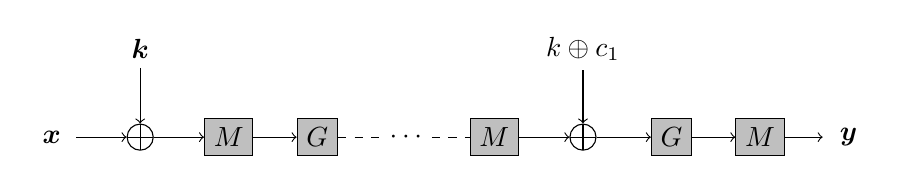
\begin{tikzpicture}[node distance={32pt}, node/.style = {draw, circle},on grid=true]
      \node[node,draw=none] (x) {\(\bm{x}\)};
      \node[xor,draw=black,fill=none] (a1) [right of=x] {};
      \node[draw=none] (c1) [above of=a1] {\(\bm{k}\)};
      \node[node,shape=rectangle,fill=lightgray] (m1) [right of=a1] {\(M\)};
      \node[node,shape=rectangle,fill=lightgray] (g1) [right of=m1] {\(G\)};
      \node (dots) [right of=g1] {\(\cdots \)};
      \node[node,shape=rectangle,fill=lightgray] (m2) [right of=dots] {\(M\)};
      \node[xor,draw=black,fill=none] (a2) [right of=m2] {};
      \node[draw=none] (c2) [above of=a2] {\(k \oplus c_1\)};
      \node[node,shape=rectangle,fill=lightgray] (g2) [right of=a2] {\(G\)};
      \node[node,shape=rectangle,fill=lightgray] (m3) [right of=g2] {\(M\)};
      \node[node,draw=none] (y) [right of=m3] {\(\bm{y}\)};

      \draw[->] (x) to (a1);
      \draw[->] (c1) to (a1);
      \draw[->] (a1) to (m1);
      \draw[->] (m1) to (g1);
      \draw[dashed,-] (g1) to (dots);
      \draw[dashed,-] (dots) to (m2);
      \draw[->] (m2) to (a2);
      \draw[->] (c2) to (a2);
      \draw[->] (a2) to (g2);
      \draw[->] (g2) to (m3);
      \draw[->] (m3) to (y);
    \end{tikzpicture}
  \end{figure}

  \Arion{}, a new keyed permutation from the GTDS\@:
  \begin{itemize}
    \item Exponent \(d_2\): inverse is large, few constraints for exponentiation.
    \item Affine layer: matrix with linear matrix-vector product complexity. 
    \item Achieves degree overflow in just one round.
    \item \Arionp{}: one-way permutation obtained from fixed-key \Arion{}. 
  \end{itemize}
\end{frame}

\begin{frame}{\Arionhash{} and \Aarionhash{}}
  \begin{figure}
    \centering
    \includegraphics[scale=0.5]{res/SpongeConstruction.pdf}
  \end{figure}

  The \Arionhash{} hash function:
  \begin{itemize}
    \item Derived from \Arionp{} in \textbf{sponge mode}~\cite{BertoniDPA2007}.
    \item \Arionhash{}-256: only \textbf{76 R1CS constraints}.
    \item \(330\times \) less than SHA-256!
    \item \(3.2\times \) less than \Poseidon{}, \(25\% \) less than \Griffin{}.
  \end{itemize}
\end{frame}

\begin{frame}{Experiments}
  %  \begin{figure}
  %    \centering
  %    \includegraphics[scale=0.2]{res/libsnark.png}
  %  \end{figure}
  \begin{table}
    \centering
    \caption*{Proof generation times for Merkle commitments over the BN-254~\cite{BarretoN2005} field.}
        \begin{tabular}{c | c c c c}  
          \toprule
          Tree height & \(\bm{\alpha}\)\textbf{-ArionHash} & \Griffin{} & \Poseidon{} & \Mimc{} \\
          \midrule
          \(4\)   & \(\bm{73}\) ms  & \(88\) ms & \(186\) ms   & \(350\)  ms \\
          \(8\)   & \(\bm{145}\) ms & \(181\) ms & \(386\) ms  & \(735\)  ms \\
          \(16\)  & \(\bm{278}\) ms & \(338\) ms & \(745\) ms  & \(1460\) ms \\
          \(32\)  & \(\bm{509}\) ms & \(622\) ms & \(1422\) ms & \(2930\) ms \\
          \bottomrule
        \end{tabular}
  \end{table}
  \vspace*{16pt}
  \texttt{libsnark}: standard C\texttt{++} library for ZK-SNARK (ZCash~\cite{SassonCGGMTV2014}).\\
  I used it to write a library containing:
  \begin{itemize}
    \item \Arion{} and other arithmetization-oriented cryptographic primitives.
    \item A self-configuring Merkle tree, and the ABR mode~\cite{AndreevaBR2021}.
    \item A unified interface to write, test and benchmark new designs.
    \item Will be open-sourced once the article is published.
  \end{itemize}
\end{frame}

\begin{frame}
  \begin{center}
    \rule{\textwidth}{0.5pt}
    \huge{\(\mathcal{T}\mathit{he}\)} \ \huge{\(\mathcal{E}\mathit{nd}\)}\\
    \Large{\emph{Thank you for your attention!}}
    \rule{\textwidth}{0.5pt}
  \end{center}
\end{frame}

\section{Extra}

\begin{frame}[noframenumbering]{The Augmented Binary tRee~\cite{AndreevaBR2021}}
  \begin{figure}
    \centering
    \adjustbox{max height=128pt,keepaspectratio}{
      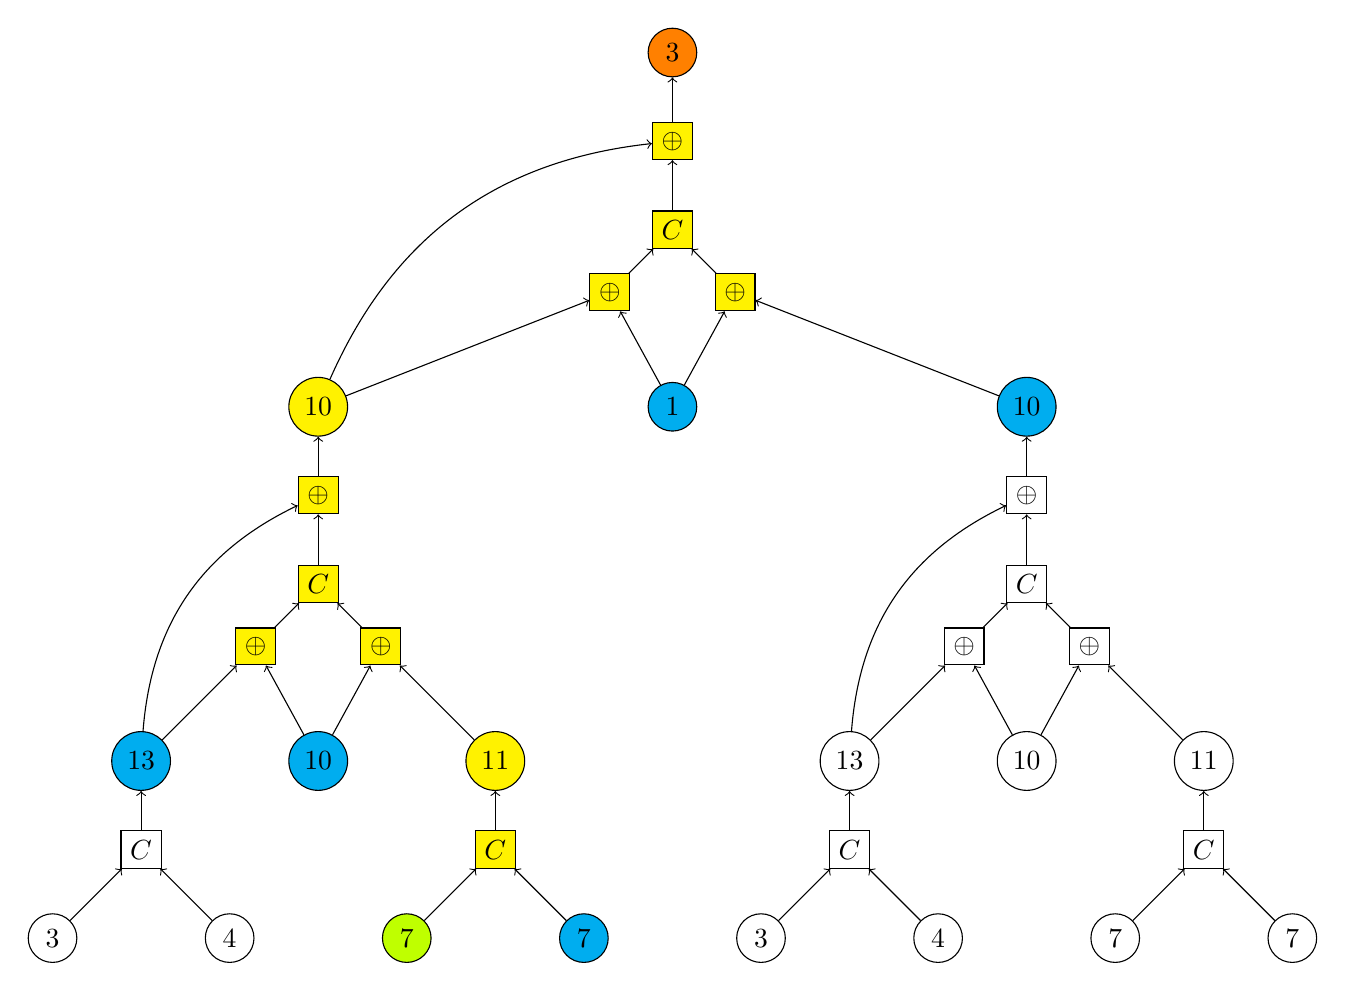
\begin{tikzpicture}[node distance={32pt}, node/.style = {draw, circle},on grid=true]
        \node[node] (x1) {\(3\)};
        \node[node,draw=none] (n1) [right of=x1] {};
        \node[node] (x2) [right of=n1] {\(4\)};
        \node[node,shape=rectangle] (c1) [above of=n1] {\(C\)};
        \node[node,draw=none] (n2) [right of=x2] {};
        \node[node,fill=lime] (x3) [right of=n2] {\(7\)};
        \node[node,draw=none] (n3) [right of=x3] {};
        \node[node,fill=cyan] (x4) [right of=n3] {\(7\)};
        \node[node,shape=rectangle,fill=yellow] (c2) [above of=n3] {\(C\)};
        \node[node,draw=none] (n4) [above of=n2] {};
        \node[node,fill=cyan] (x8) [above of=n4] {\(10\)};
        \node[node,fill=cyan] (x5) [above of=c1] {\(13\)};
        \node[node,fill=yellow] (x6) [above of=c2] {\(11\)};
        \node[node,draw=none] (n5) [above of=x8] {};
        \node[node,shape=rectangle,fill=yellow] (c3) [above of=n5] {\(C\)};
        \node[node,shape=rectangle,fill=yellow] (a1) [below left of=c3] {\(\oplus \)};
        \node[node,shape=rectangle,fill=yellow] (a2) [below right of=c3] {\(\oplus \)};
        \node[node,shape=rectangle,fill=yellow] (a3) [above of=c3] {\(\oplus \)};
        \node[node,fill=yellow] (x7) [above of=a3] {\(10\)};

        \draw[->] (x1) to (c1);
        \draw[->] (x2) to (c1);
        \draw[->] (x3) to (c2);
        \draw[->] (x4) to (c2);
        \draw[->] (c1) to (x5);
        \draw[->] (c2) to (x6);
        \draw[->] (x5) to (a1);
        \draw[->] (x6) to (a2);
        \draw[->] (x8) to (a1);
        \draw[->] (x8) to (a2);
        \draw[->] (a1) to (c3);
        \draw[->] (a2) to (c3);
        \draw[->] (c3) to (a3);
        \draw[->] (x5) [bend left] to (a3);
        \draw[->] (a3) to (x7);

        \node[node,draw=none] (n0) [right of=x4] {};
        \node[node] (y1) [right of=n0] {\(3\)};
        \node[node,draw=none] (n1) [right of=y1] {};
        \node[node] (x2) [right of=n1] {\(4\)};
        \node[node,shape=rectangle] (c1) [above of=n1] {\(C\)};
        \node[node,draw=none] (n2) [right of=x2] {};
        \node[node] (x3) [right of=n2] {\(7\)};
        \node[node,draw=none] (n3) [right of=x3] {};
        \node[node] (x4) [right of=n3] {\(7\)};
        \node[node,shape=rectangle] (c2) [above of=n3] {\(C\)};
        \node[node,draw=none] (n4) [above of=n2] {};
        \node[node] (x8) [above of=n4] {\(10\)};
        \node[node] (x5) [above of=c1] {\(13\)};
        \node[node] (x6) [above of=c2] {\(11\)};
        \node[node,draw=none] (n5) [above of=x8] {};
        \node[node,shape=rectangle] (c3) [above of=n5] {\(C\)};
        \node[node,shape=rectangle] (a1) [below left of=c3] {\(\oplus \)};
        \node[node,shape=rectangle] (a2) [below right of=c3] {\(\oplus \)};
        \node[node,shape=rectangle] (a3) [above of=c3] {\(\oplus \)};
        \node[node,fill=cyan] (y7) [above of=a3] {\(10\)};
        \node[node,draw=none] (n6) [above of=n0] {};
        \node[node,draw=none] (n7) [above of=n6] {};
        \node[node,draw=none] (n8) [above of=n7] {};
        \node[node,draw=none] (n9) [above of=n8] {};
        \node[node,draw=none] (n10) [above of=n9] {};
        \node[node,fill=cyan] (y8) [above of=n10] {\(1\)};
        \node[node,draw=none] (n11) [above of=y8] {};
        \node[node,shape=rectangle,fill=yellow] (c4) [above of=n11] {\(C\)};
        \node[node,shape=rectangle,fill=yellow] (a4) [below left of=c4] {\(\oplus \)};
        \node[node,shape=rectangle,fill=yellow] (a5) [below right of=c4] {\(\oplus \)};
        \node[node,shape=rectangle,fill=yellow] (a6) [above of=c4] {\(\oplus \)};
        \node[node,fill=orange] (z) [above of=a6] {\(3\)};
       
        \draw[->] (y1) to (c1);
        \draw[->] (x2) to (c1);
        \draw[->] (x3) to (c2);
        \draw[->] (x4) to (c2);
        \draw[->] (c1) to (x5);
        \draw[->] (c2) to (x6);
        \draw[->] (x5) to (a1);
        \draw[->] (x6) to (a2);
        \draw[->] (x8) to (a1);
        \draw[->] (x8) to (a2);
        \draw[->] (a1) to (c3);
        \draw[->] (a2) to (c3);
        \draw[->] (c3) to (a3);
        \draw[->] (x5) [bend left] to (a3);
        \draw[->] (a3) to (y7);

        \draw[->] (x7) to (a4);
        \draw[->] (y8) to (a4);
        \draw[->] (y7) to (a5);
        \draw[->] (y8) to (a5);
        \draw[->] (a4) to (c4);
        \draw[->] (a5) to (c4);
        \draw[->] (c4) to (a6);
        \draw[->] (x7) [bend left] to (a6);
        \draw[->] (a6) to (z);

        
 
      \end{tikzpicture}
    }
  \end{figure}

  \begin{itemize}
    \item \emph{Compactness} \(\approx \) blocks compressed per function call.
    \item Merkle Tree compactness is \(2/3\). 
    \item ABR interleaves OWCF calls with field addition.
    \item ABR processes 50\% more messages: compactness is \(1\).
    \item Additions are basically free in ZK-SNARK\@!
  \end{itemize}
\end{frame}

\begin{frame}[noframenumbering]{Experimental results}
  ABR vs.\ Merkle Tree relative performance for increasing height:
  \begin{figure}
    \centering
    \includegraphics[scale=0.25]{res/abr_vs_mtree.png}
  \end{figure}
\end{frame}

\begin{frame}[allowframebreaks,noframenumbering]
  \bibliographystyle{alpha}
  \bibliography{biblio.bib}
\end{frame}
\end{document}
